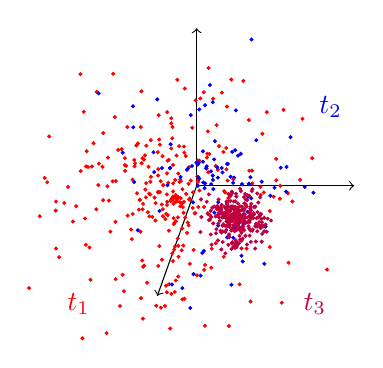
\begin{tikzpicture}
    [   cnode/.style={draw=black,fill=#1,minimum width=3mm,circle},
        rnode/.style={draw=#1!40,fill=#1!20,minimum width=6mm, minimum height=6mm, rectangle}
    ]
    
    \draw [->] (0, 0) -- (0, 2);
    \draw [->] (0, 0) -- (2, 0);
    \draw [->] (0, 0) -- (-0.5, -1.4);
    
    \draw [red] plot [only marks, draw=red, mark=*, mark size=0.5, domain=0:2, samples=300] ({4*(rnd-0.5)*rnd-0.3},{4*(rnd-0.5)*rnd-0.2});
    
    \draw [blue] plot [only marks, draw=red, mark=*, mark size=0.5, domain=0:2, samples=100] ({3*(rnd-0.5)*rnd+0.1},{4*(rnd-0.5)*rnd+0.1});
    
    \draw [purple] plot [only marks, draw=red, mark=*, mark size=0.5, domain=0:2, samples=300] ({1*(rnd-0.5)*rnd+0.5},{1*(rnd-0.5)*rnd-0.4});
    
    \node [red] at (-1.5, -1.5) {$t_1$};
    \node [blue] at (1.7, 1) {$t_2$};
    \node [purple] at (1.5, -1.5) {$t_3$};
    \end{tikzpicture}